%%% Template para anotações de aula
%%% Feito por Daniel Campos com base no template de Willian Chamma que fez com base no template de  Mikhail Klassen


\documentclass[12pt,a4paper, brazil]{article}

%%%%%%% INFORMAÇÕES DO CABEÇALHO
\newcommand{\workingDate}{\textsc{\selectlanguage{portuguese}\today}}
\newcommand{\userName}{QXD0115 \textbf{-} EDA}
\newcommand{\institution}{UFC-QX}
\usepackage{researchdiary_png}
\usepackage{comment}
\usepackage{xcolor}
\usepackage{graphics}

%%---------{Meus Comandos}---------%%
\newcommand{\B}[1]{\textbf{#1}}
\newcommand{\azul}[1]{\textcolor{blue}{#1}}
\newcommand{\vermelho}[1]{\textcolor{red}{#1}}
\newcommand{\verde}[1]{\textcolor{green}{#1}}
\begin{document}

\begin{center}
{\textbf {\huge Problemas 1, 2 e 3\\(Trabalho Grafos)}}\\[5mm]
{\large Gustavo Gurgel Medeiros} \\[5mm]
\today\\[5mm] %% se quiser colocar data
\end{center}

\section{(Porblema 1) (Código em C++) Usando \emph{Duas} Cores, Dizer se Existe Coloração Válida do Grafo.}

\subsection{Interpretação e resolução do Problema}

Na questão foi pedido a implementação de um \B{código em c++} que, dado um grafo $G=(V,E)$ qualquer e usando \B{duas cores}, retorna se é possível colorir todos os vértices de maneira que vértices vizinhos não possuam a mesma cor. Um pensamento válido para se colorir esse grafo seria fazer uma divisão de seus vértices em 2 \emph{conjuntos disjuntos} $V_1$ e $V_2$, sendo que toda aresta em $E$ tem uma extremidade em $V_1$ e outra em $V_2$. E assim, colorir um conjunto com uma \azul{cor1} e ou outro com uma \vermelho{cor2}. Como os dois conjuntos são disjuntos e pela nossa definição as arestas não podem ter extremidade no mesmo cojunto, então coloração seria válida. Um grafo que sitisfaz esse propriedade é dito grafo bipartido. Consequentemente, uma grafo tem coloração válida se somente se ele for bipartido. \\[1mm] 

\noindent Fazendo a aplicação desta interpretação para o seguinte grafo com	 $|V|=4$:
 
\begin{center}
	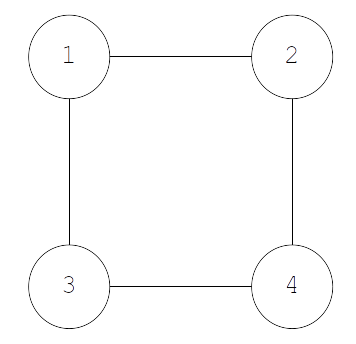
\includegraphics[scale=0.5]{grafo4.png}
\end{center}

\newpage

\noindent Dividindo o grafo da maneira que foi proposto chegamos ao seguinte resultado:

\begin{center}
	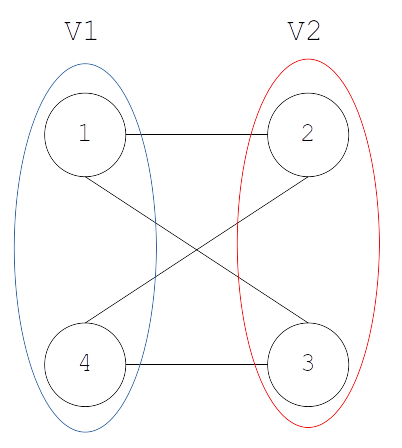
\includegraphics[scale=0.45]{grafo4-b.png}
\end{center}

Como pode ser visto o grafo foi devidamente pintado. Logo, para dizer se é possível pintar o grafo com duas cores, basta descobrir se ele é bipartido ou não. Para isso temos que achar ciclos de tamanho ímpar. Se um grafo não tem ciclo de tamanho ímpar, então ele é bipartido. Isso acontece pois sempre que temos um ciclo de tamanho ímpar, temos um vértice que conecta duas extremidades de um caminho par. Como para todo caminho par suas extremidades vão ter cores diferentes, qualquer que seja a cor do vértice que conecta essas duas extremidades vai violar nossa propriedade. Isso fica bem ilustrado na imagem abaixo:

\begin{center}
	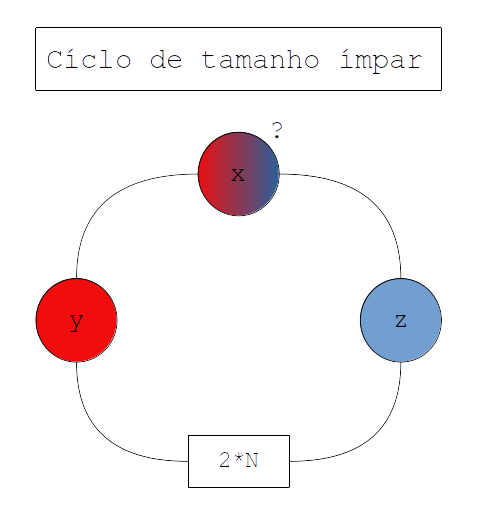
\includegraphics[scale=0.45]{bipartido.png}
\end{center} 

\newpage

Portanto, finalizando o raciocínio, é preciso desenvolver um algoritmo que encontre ciclos de tamanho ímpar. Sé algum caminho de tamanho ímpar for encontrado então o grafo \B{não pode ser biparido} e consequentemente \B{não existe coloração válida}. Caso o contrário, se nenhum ciclo de tamanho impar existir, então o grafo é bipartido, assim, \B{existe uma coloração válida}.

\subsection{Explicação do algoritmo}

Para essa questão foi desenvolvida uma classe \b{Graph}, que representa um grafo utilizando listas de adjacências. Como a classe é simples, não vejo necessidade de documentar todas as suas propriedades aqui. Dessa forma, vamos focar no método principal que resolve o problema passado pela questão. Esse método é o \azul{canBeColored()} que retoma um valor booleano para se existe ou não coloração válida.

Para achar ciclos de tamanho impar, a função \azul{canBeColored()} utiliza \B{busca por profundidade}. Dois vetores são usados, um para armazenar as \B{cores} de cada vértice, e outro para armazenar a \B{distância percorrida} da origem até o vértice em questão, sendo que a origem tem distância 0 dela mesma. Assim, após os vetores de cores e distâncias serem inicializados com os valores branco e 0 respectivamente, um loop é iniciado para definir uma origem (um vértice branco) a ser explorada. Depois que a origem $u$ é definida, um loop de exploração começa a fazer a busca por profundidade em todos os vértices conexos a $u$. Se em algum momento da busca um vértice cinza possuir um outro vértice cinza adjacente a ele, então é porque temos um ciclo no grafo. Calculamos a distância absoluta entre esses dois vértices e isso retoma a quantidade de aresta entre os dois. Essa distância é somada +1, pois existe uma aresta a mais que conclui o ciclo. Se essa ao final da conta essa distância for um \B{valor maior que dois e impar}, então achamos um ciclo de tamanho impar. Consequentemente o grafo não pode ser bipartido, logo a função retorna \vermelho{false}. Se após exploração completa do grafo não forem encontrado ciclos de tamanho ímpar, então o \B{grafo é bipartido} e consequentemente existe coloração válida, assim a função retorna \verde{true}. Assim, finalizamos a explicação do algoritmo implementado.

\subsection{Analise de complexidade de tempo e espaço}

Para esse algoritmo, o pior caso é quando \B{existe uma coloração valida}, pois neste caso a busca por profundidade vai rodar até o final, até que não se ache ciclos de tamanho impar. Com isso, como já foi discutido em sala, para a busca em profundidade sua complexidade de tempo é da ordem de $\mathcal{O}(|V|+|E|)$. Além disso, como estamos representando o grafo como uma lista de adjacência, o espaço utlizado também é da ordem de $\mathcal{O}(|V|+|E|)$.
\section{(Porblema 2) (Código em C++) Calcular "Número de Bacon" de atores}

\subsection{Interpretação e resolução do Problema}

A interpretação desse problema é de certa maneira simples. Dado um grafo de atores que representa as relações entre atores que fizeram os mesmos filmes, precisamos encontrar o \B{número de bacon} de todos os atores. O número de bacon é representado pelo \B{menor caminho entre Kevin Bacon e um vértice qualquer do grafo}. Quando pensamos em menor caminho, busca em largura parece ser uma alternativa viável. Isso porque dado uma origem $u$ qualquer e um vértice $v$. Se existir uma caminho entre $u$ e $v$, então a busca em largura vai retorna a caminho mínimo entre $u$ e $v$. Como esse teorema esse já foi provado em sala e nos slides, não vou refazer a prova aqui. Sabendo disso, uma resolução pare esse algoritmo seria criar o grafo de relações de Atores e chamar a busca em largura tendo Kevin Bacon como origem. Dessa forma, Kevin Bacon tem número de bacon $0$ e todo vértice adjacente a ele tem número de bacon $= 0+1$ e vértices adjacentes a vértices adjacentes a Kevin Bacon tem número de bacon $=1+1$ e assim por diante. Após isso, armazenamos todos esses valores em uma tabela e fazemos a impressão.

\subsection{Explicação do algoritmo}

Para mim, o desafio principal dessa questão não foi calcular o número de bacon, mas sim representa o grafo de Atores. Até então, cada grafo era representado por um valor numérico. Dessa forma era possível fazer a lista de adjacência apenas como um vetor de acesso direto. Porém, agora como cada vértice do grafo seria representado por um ator, foi necessário adaptar a antiga implementação. Assim, para contorna a não possibilidade de acesso direto, mas ainda efetuar inserções e requisições em média de tempo $\mathcal{O}(1)$, a lista de adjacência foi implementada como uma \azul{HashTable<K,T>}, sendo que K é uma string representado o \B{nome do ator} e T sendo uma lista de \B{structs do tipo Actor}. Veja a implementação abaixo: 

\begin{center}
	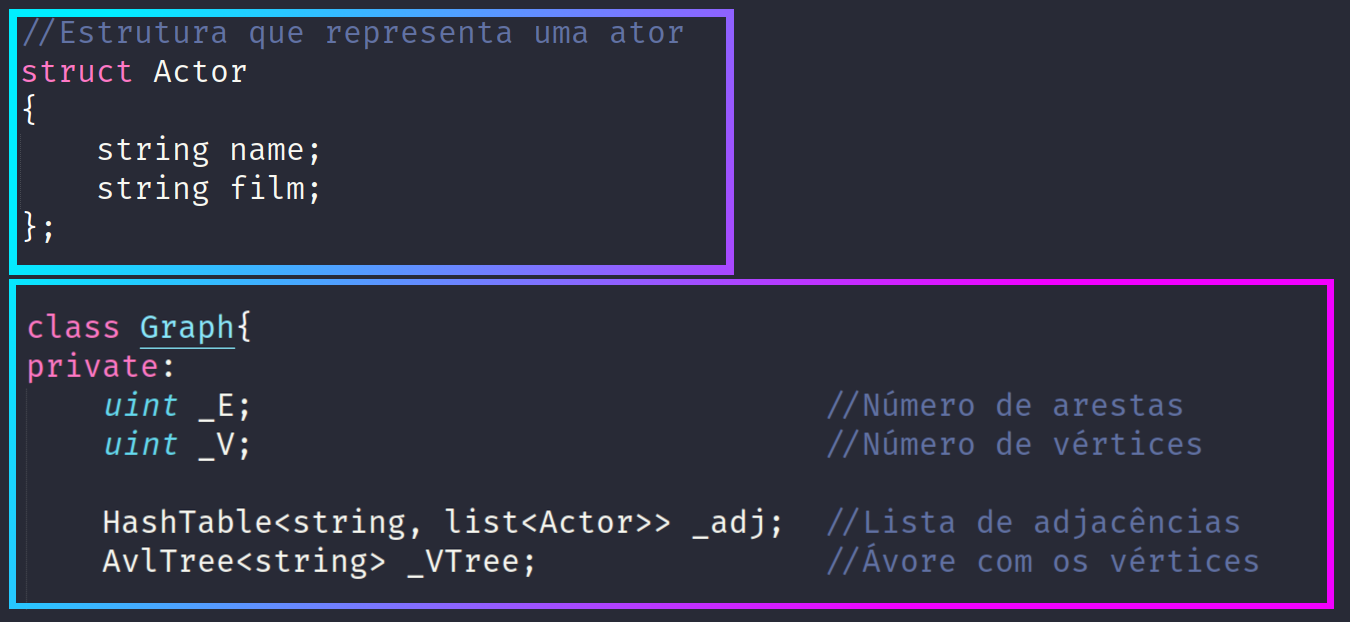
\includegraphics[scale=0.35]{classgraph.png}
\end{center}

Perceba que necessidade da struct Actor surge pois o vértice que conecta dois atores tem uma informação extra, que no caso é o nome do filme que os dois participaram. Essa informação precisa ser guardada pois problema pede que além do número de bacon do ator, seja passado o filme pelo qual ele recebe esse número. Além disso, como os vértices não pertencem a um intervalo inteiro, é preciso guardar os vértices que foram adicionados no grafo de forma que não tenham vértices duplicados. Com isso, pensando em uma estrutura de dados que não permita elementos duplicados e inserções em tempo logarítmico, eu decidi utilizar uma árvore AVL. Essa estrutura ajuda ainda mais, pois pelo fato de ela ser uma árvore binária de busca, pode-mos usar inorder para pegar os elementos ordenados em tempo linear. Isso casa perfeitamente com o fato da saída do programa ser o número de bacon dos vértices em ordem alfabética.

Para adicionar elementos no grafo eu fiz uma função chamada \azul{halfInsert(u, v)}, que dados dois atores u e v a função adiciona apenas a aresta unidirecional de $u \rightarrow v$. Assim, na função pública insert(u,v), halfInsert é chamado duas vezes adicionado as arestas $u \rightarrow v$ e $v \rightarrow u$. Isso pode ser analisado na implementação abaixo:

\begin{center}
	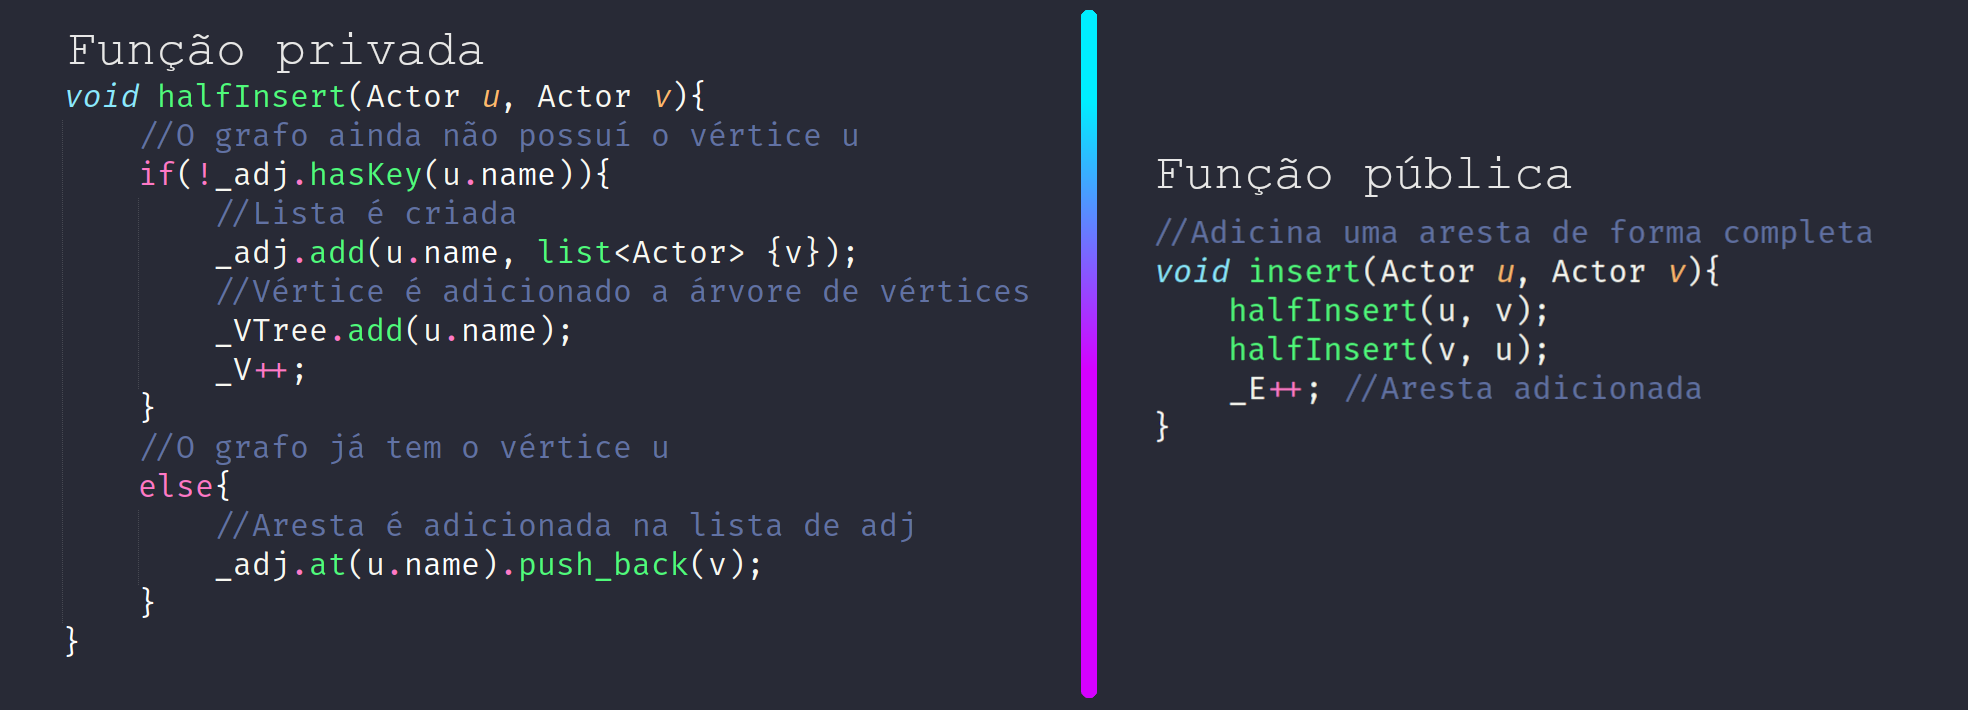
\includegraphics[scale=0.25]{insert.png}
\end{center}

Perceba que função \azul{halfInsert(u, v)} analisa se na HashTable já existe a lista de adjacência com a \B{key = nome\_ator}. Se sim, então ele só adiciona na lista já existente, caso o contrário a lista para aquela chave e criada e o vértice é adicionado a árvore.

Agora, vamos falar da função \azul{getBaconTable}. Essa função é a que de fato resolve o problema em questão. Veja o ínicio da sua declaração abaixo:

\begin{center}
	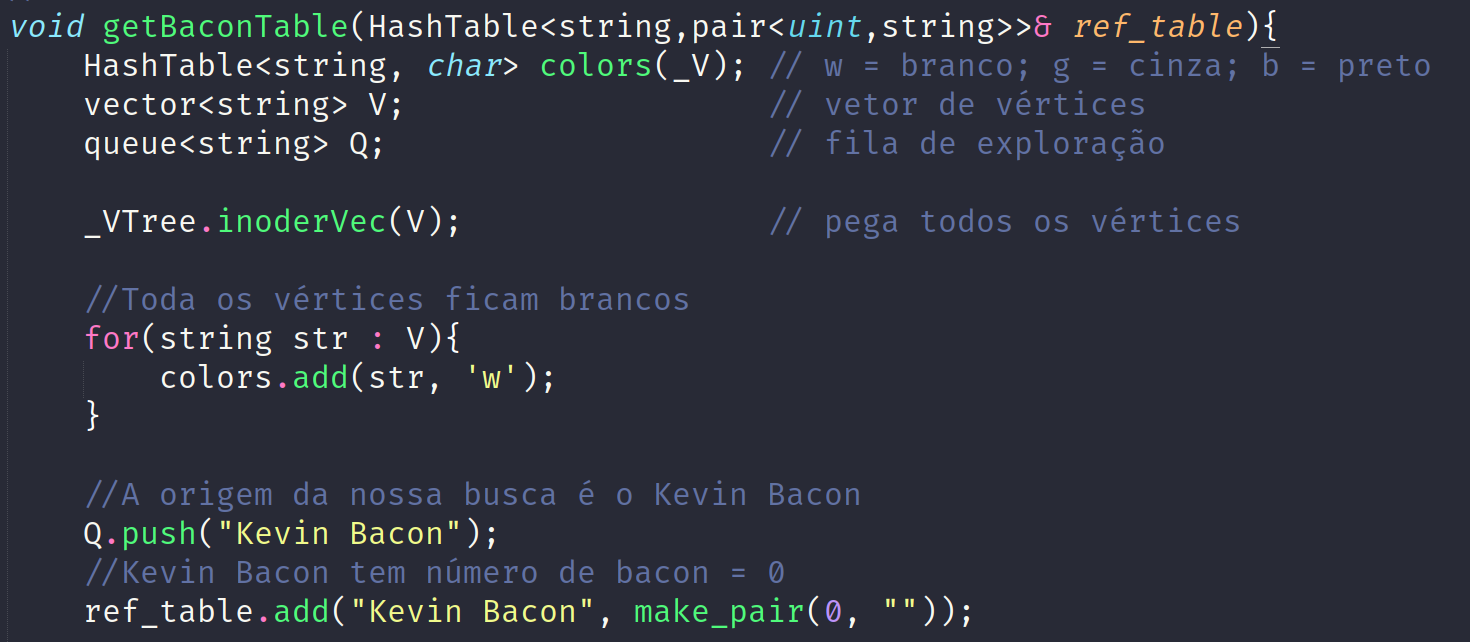
\includegraphics[scale=0.33]{bacontable1.png}
\end{center}

Essa função recebe uma referência a uma HashTable do tipo \vermelho{<string, pair<uint, string>>} e vai adicionar elementos de tal forma que no final da função todo vértice (nome de ator) do grafo seja uma chave ligada a um par de elementos, sendo primeiro o número de bacon e o segundo o nome do filme pelo qual o vértice recebe esse número. Além disso, a função cria uma HashTable auxiliar que vai representar as cores de cada vértice na tabela. Após isso, Kevin Bacon é adicionando em uma queue para ser a origem da nossa busca. Como é possível ver abaixo, a busca por largura se inicia e adicionamos na tabela os pares relacionados a cada cada ator:
	
\begin{center}
	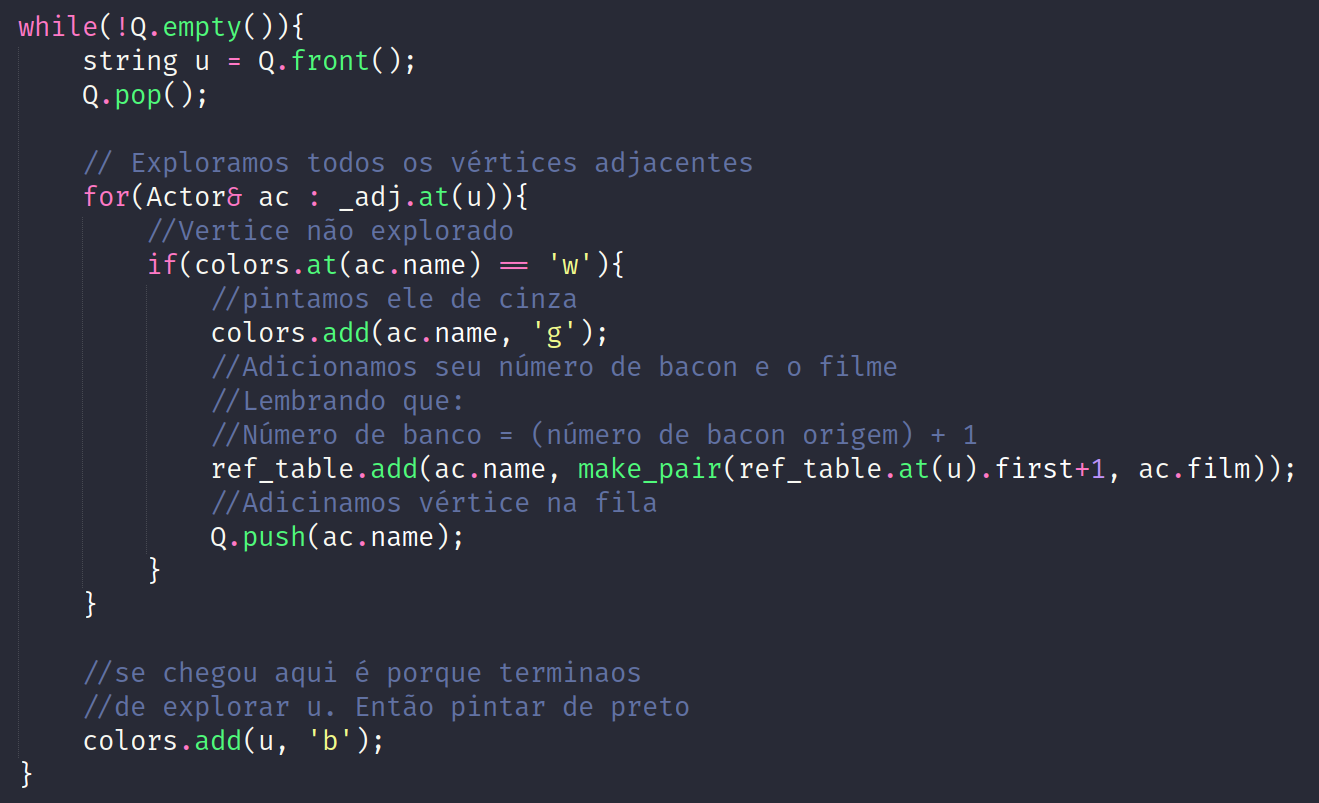
\includegraphics[scale=0.33]{bacontable2.png}
\end{center}	

Ao final, a tabela passado como referência vai conter para todo nome de ator, seu número de bacon e filme que faz ele receber esse número. Após isso, o resto da implementação é apenas leitura e escrita de dados na main, que não vou debater aqui. Concludentemente, a explicação da implementação é para esse problema é finalizada.

\subsection{Analise de complexidade de tempo e espaço}
Para esse algoritmo, creio que a função principal é a \azul{getBaconTable}, considerando apenas a busca em largura para essa função e levando em conta que os acessos a tabela de cores é em média $\mathcal{O}(1)$, então como já foi debatido em sala e nos slides, a complexidade para esse busca é da ordem de $\mathcal{O}(|V|+|E|)$. Em questão de utilização espaço, a lista de adjacência usa $\mathcal{O}(|V|+|E|)$ de espaço e a árvore AVL que guarda todos os vértices $\mathcal{O}(|V|)$.

\section{(Porblema 3) (Código em C++) Converter ruas de mão dupla em mão única com caminho para qualquer cidade}

\subsection{Interpretação e resolução do Problema}

Nessa questão foi pedido que, dado um grafo não direcionado que representa as ruas de mão dupla de uma cidade, fosse convertido todas as ocorrências possíveis de vias de mão dupla em mão única. Ou seja, o que devemos fazer é pegar um grafo não direcionado e de alguma forma torna para maioria dos vértices o grau de entrada e saída em 1. Pensando nisso, a primeira ideia que eu tive foi ''caminhar/explorar'' de alguma forma o grafo e fazer ligações entre os vértices. Assim, uma das alternativas seria fazer busca por largura ou profundidade e criar um novo grafo para guardar o resultado dessa busca. Porém, fica a dúvida, \azul{qual das duas buscas é melhor para o nosso problema?}. Vamo fazer uma uma comparação para seguinte grafo:


\begin{center}
	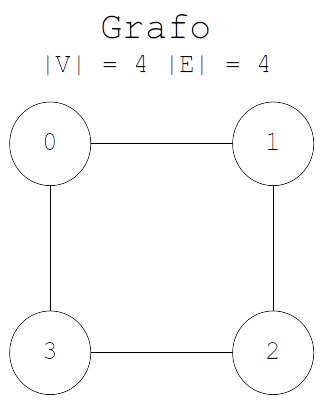
\includegraphics[scale=0.6]{grafo-qs3.png}
\end{center}

\noindent Um resultado válido para a busca em largura tendo como origem o vértice 0:

\begin{center}
	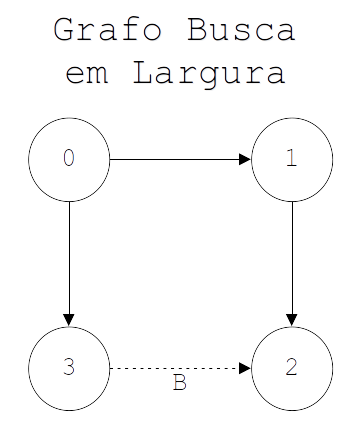
\includegraphics[scale=0.6]{grafo-qs3-bel.png}
\end{center}

\newpage

\noindent Um resultado válido para a busca em profundidade tendo como origem o vértice 0:

\begin{center}
	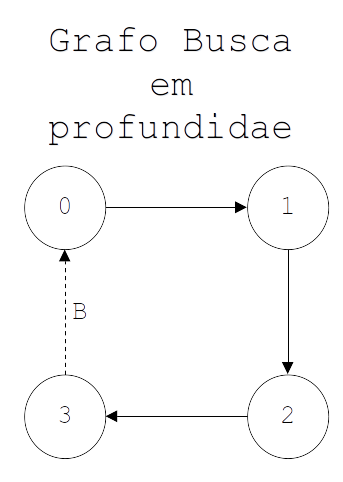
\includegraphics[scale=0.6]{grafo-qs3-bep.png}
\end{center}

Perceba que busca em profundidade produz um caminho mais linear que a busca em largura. Além disso, se consideramos os backedges podemos criar grafos com ciclos de pistas únicas, o que encaixa perfeitamente na questão.

Com isso, chegamos que uma possível solução para o problema. Porém, perceba que ainda existe uma complicação a ser resolvida. Para muitos grafos, quando adotamos essa metodologia, a conversão acaba criando componentes fortemente conexas, ou seja, subgrupos de vértices que tem caminho para todos elementos dentro grupo, mas não para elementos fora do grupo.\\[2mm]

\noindent Um exemplo bem claro disso pode ser visto se metodologia for aplicada para o seguinte grafo:\\

\begin{center}
	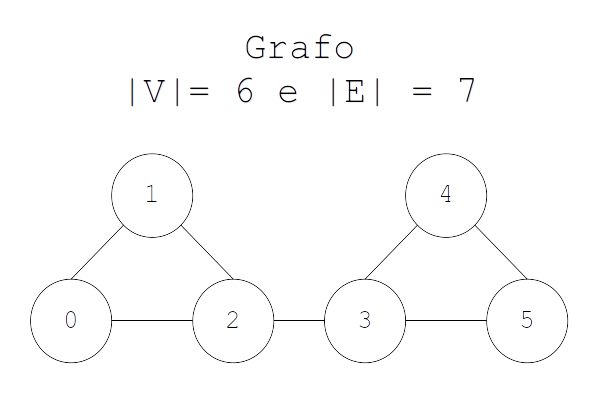
\includegraphics[scale=0.4]{grafo5.png}
\end{center}

\newpage

Depois da conversão temos a seguinte análise: \\

\begin{center}
	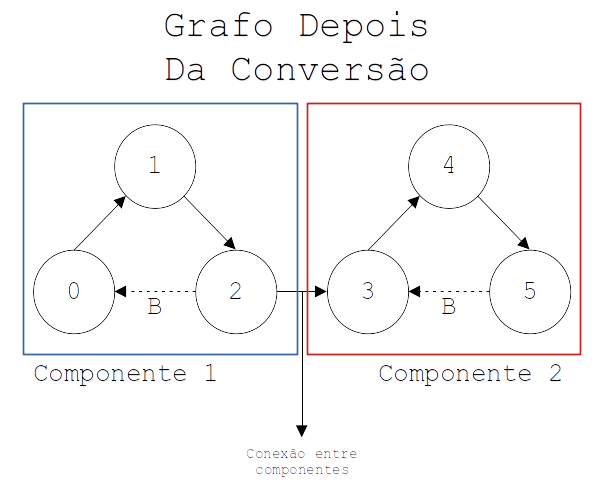
\includegraphics[scale=0.6]{grafo-depois.png}
\end{center}

Perceba que as componentes têm caminhos entre todos seus vértices, porém temos apenas um caminho de ida da componente 1 a 2. Por isso para todas as componentes precisamos fazer conexão de ida e volta. Ficando com o seguinte grafo

\begin{center}
	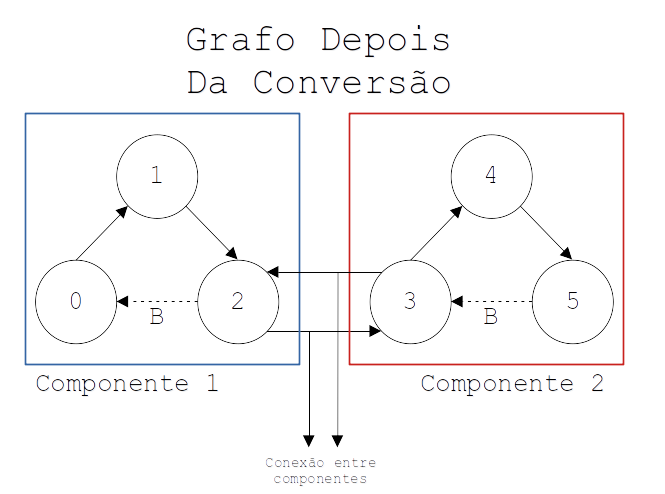
\includegraphics[scale=0.6]{grafo-depois-2.png}
\end{center}

Depois de conectar as componentes obtemos o gráfico da maneira que a questão pede. Assim, concluímos o desenvolvimento da solução do problema.

\subsection{Explicação do algoritmo}

\noindent Nessa questão vou explicar o algoritmo descrevendo os métodos principais da classe grafo que resolve o problema. Isso porque eu acho que o procedimento para resolver o problema já foi explicado muito bem no tópico anterior:

\begin{enumerate}
	\item \azul{malformedConvert()} 
		\begin{itemize}
			\item Usa busca por profundidade para criar o grafo direcionado. Considerando backedges para criar ciclos e componentes
			\item Essa função faz uma espécie de conversão ''malformada'' do grafo, sem conexões entre as componentes.
			\item É uma função privada pois é apenas de uso interno da clase graph.
		\end{itemize}
	\item \azul{getComponents()} 
		\begin{itemize}
			\item Retorna um vetor com as componentes de um grafo direcionado
			\item usa o Kosaraju's Algorithm (tempo $\mathcal{O}(|V|+|E|)$)
		\end{itemize}
	\item \azul{convertInDirected()} 
		\begin{itemize}
			\item Função principal que resolve o problema da questão
			\item Essa função usa ambas as funções citadas anteriormente. Pirmeiramente ele pega a forma malformada do grafo que chamou o método. Depois usa função getComponents para pegar as componentes do grafo malformado. Por fim, faz uma busca em profundidade pelo grafo e  conserta todos as arestas que ligam componentes do grafo, da mesma forma que foi debatido nó tópico de intepretação dessa questão.
		\end{itemize}
	
\end{enumerate}

\subsection{Analise de complexidade}

Nessa questão a funções principais são a malformedConvert(), getComponents() e convertInDirected(). Como já foi dito no tópico anterior a função getComponents() usa o \B{Kosaraju's Algorithm} que internamente usa busca em profundidade para encontrar as componentes, ou seja, sua complexidade é $\mathcal{O}(|V|+|E|)$. Da mesma forma, a função malformedConvert() usa busca em profundidade para converter um grafo não direcionado em direcionado, assim, sua complexidade também é $\mathcal{O}(|V|+|E|)$. E por último a função convertInDirected() usa os dois métodos anteriores, além de fazer mais uma busca por largura para consertar as arestas que conectam componentes, lembrando que como já foi debatido em sala e nos slides, a busca em profundidade tem complexidade $\mathcal{O}(|V|+|E|)$. Finalmente, ao juntar todos esses métodos, temos um algorítimo que ao final tem complexidade de $\mathcal{O}(|V|+|E|)$. Assim, finalizamos o raciocínio da questão.

\end{document}